\section{Problem Formulation}
\label{sec:PS}
We define the setup, objective, and constraints for user-initiated machine unlearning.

\medskip
\noindent
\textbf{Setup:}
Let $\mathcal{M}_{\textit{patient}}$ be a model pre-trained on dataset $\mathcal{D}$, with mapping $f_{\mathcal{M}_{\textit{patient}}} : \mathcal{P}_{\mathcal{D}} \rightarrow \mathcal{R}_{\mathcal{D}}$, where $\mathcal{P}_{\mathcal{D}}$ and $\mathcal{R}_{\mathcal{D}}$ denote the prompt and response spaces of $\mathcal{M}_{\textit{patient}}$ over $\mathcal{D}$. A user $\mathcal{U}$ interacts with $\mathcal{M}_{\textit{patient}}$ through prompt-response pairs $(p_t, r_t)$ at each turn $t$, forming a dialogue history $H_t = \{(p_{t-k}, r_{t-k}), \ldots, (p_t, r_t)\}$ over the last $k$ turns. 

Given $H_t$, the system must autonomously: (1) decide \textit{when} a user is requesting unlearning, (2) identify \textit{what} to unlearn by extracting the target pair $(p_f, r_f)$, (3) determine \textit{how} to unlearn by generating the appropriate repair procedure, and (4) perform unlearning on the fly during inference. Before unlearning, $\mathcal{M}_{\textit{patient}}$ maps both forget and retain prompts to their corresponding responses:
\begin{equation}
f_{\mathcal{M}_{\textit{patient}}} :
\mathcal{P}_{f} \rightarrow \mathcal{R}_f \; ; \;
\mathcal{P}_{r} \rightarrow \mathcal{R}_r
\label{eq:before_unlearn}
\end{equation}
where $p_f \in \mathcal{P}_f$, $r_f \in \mathcal{R}_f$ denote forget prompts and responses, and $p_r \in \mathcal{P}_r$, $r_r \in \mathcal{R}_r$ denote retain prompts and responses.

\medskip 
\noindent
\textbf{Objective:}
The proposed framework must transform $\mathcal{M}_{\textit{patient}}$ into $\mathcal{M}_{\textit{healed}}$ such that, after execution:
\begin{equation}
f_{\mathcal{M}_{\textit{healed}}} :
\mathcal{P}_f \cancel{\rightarrow} \mathcal{R}_f \; ; \;
\mathcal{P}_r \rightarrow \mathcal{R}_r
\label{eq:after_unlearn}
\end{equation}
where $\cancel{\rightarrow}$ denotes a forgotten mapping and $\rightarrow$ denotes a preserved mapping. Specifically, for all forget prompts, the original mapping must not hold, i.e., $f_{\mathcal{M}_{\textit{healed}}}(p_f) \neq r_f \; \forall \, (p_f, r_f) \in \mathcal{D}_f$, and for all retain prompts, the original mapping must be preserved, i.e., $f_{\mathcal{M}_{\textit{healed}}}(p_r) = r_r \; \forall \, (p_r, r_r) \in \mathcal{D}_r$\footnote{Hereafter, $\mathcal{D}_r$ refers to the retain buffer ($\leq$10\% of $\mathcal{D} \setminus \mathcal{D}_f$) unless stated otherwise.}. Here, $\mathcal{D}_f = \{(p_f, r_f)\}$ is the forget set, and $\mathcal{D}_r$ is a retain buffer comprising at most 10\% of $\mathcal{D} - \mathcal{D}_f$.

\medskip
\noindent
\textbf{Constraints:}
The above objective must be achieved under two constraints: (1) \textit{training-free}: no gradient computation or backpropagation is permitted, and (2) \textit{single-sample}: the system must operate on a single target pair $(p_f, r_f)$ rather than requiring a batch of forget samples.


\begin{figure}[htbp]
    \centering
    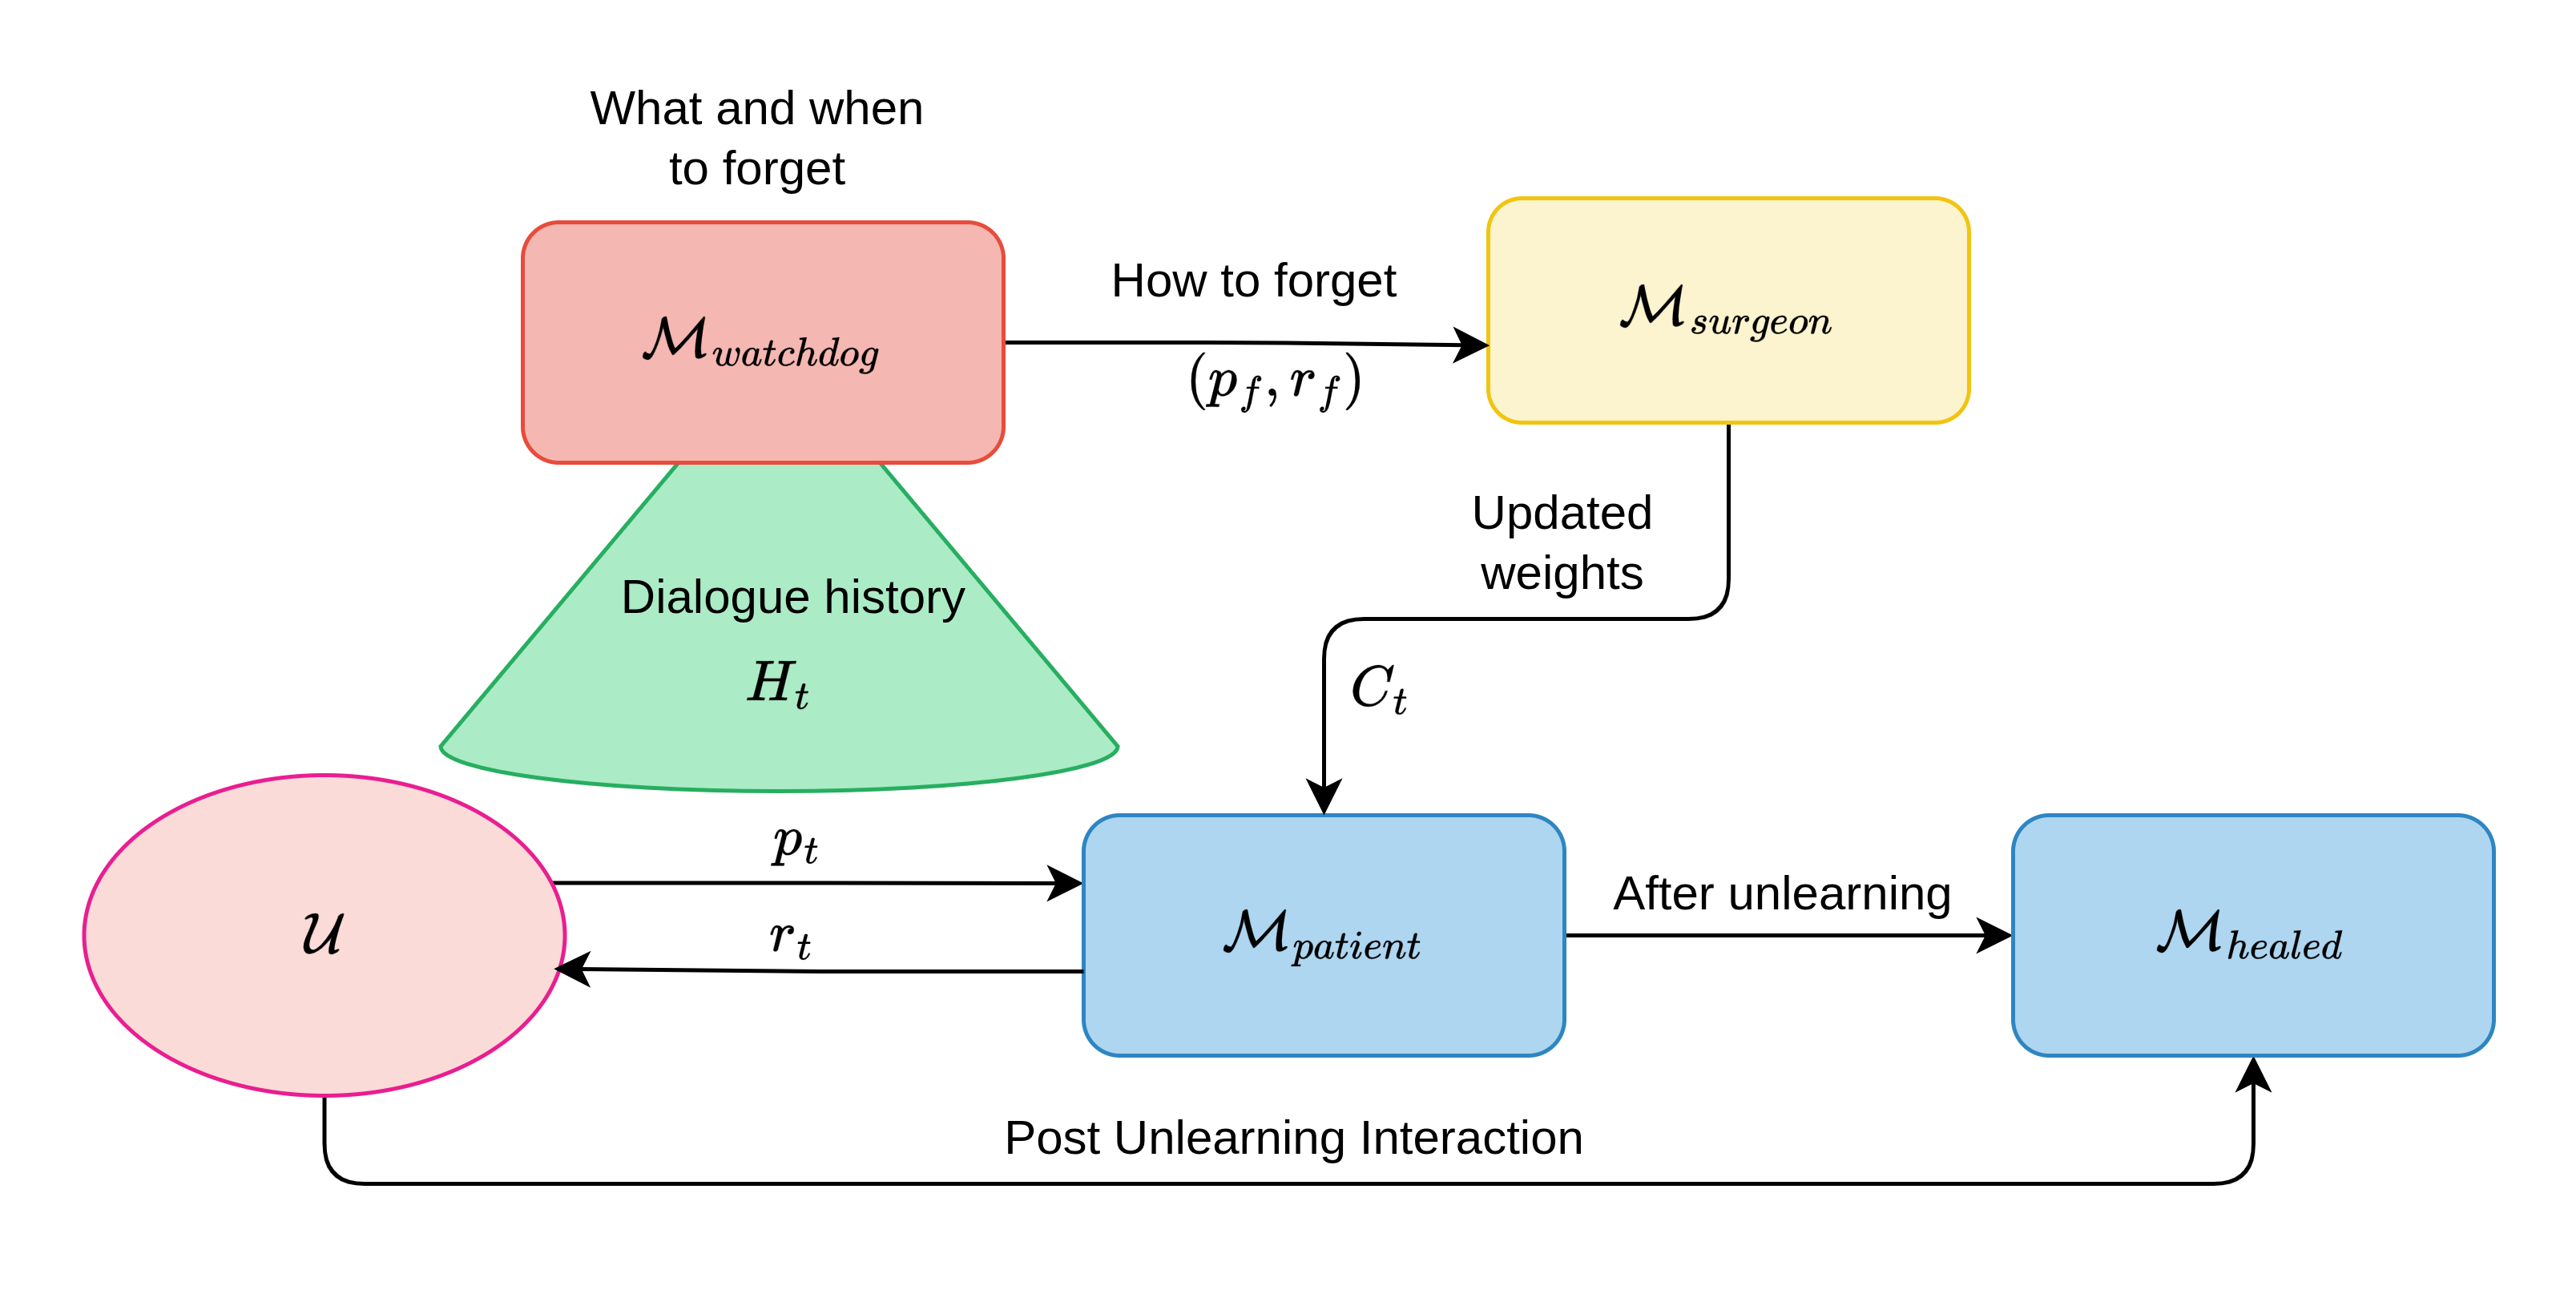
\includegraphics[width=\linewidth]{images/methodogy.png}
    \caption{Overview of the RePAIR framework. User $\mathcal{U}$ interacts with $\mathcal{M}_{\textit{\textbf{patient}}}$ via prompts $p_t$ and responses $r_t$. $\mathcal{M}_{\textit{\textbf{watchdog}}}$ detects unlearning requests from $H_t$, forwards $(p_f, r_f)$ to $\mathcal{M}_{\textit{\textbf{surgeon}}}$, which generates $C_t$ to transform $\mathcal{M}_{\textit{\textbf{patient}}}$ into $\mathcal{M}_{\textit{\textbf{healed}}}$.}
    \label{fig:framework}
\end{figure}